\documentclass[12pt,a4paper]{article}
\usepackage{enumerate} 	% put in numbers or bullet points
\usepackage{setspace}	% line spacing					
\usepackage{authblk}	% For author affiliations
\usepackage{graphicx} 	% For adding pictures
\usepackage{pdflscape}	% for landscape pages
\usepackage{mathtools}	% For equations etc.
\usepackage[osf]{mathpazo} 
\usepackage{float}		
\floatstyle{plaintop} 	% Force table captions to go above the table
\usepackage{longtable}
\usepackage[margin ={2cm, 2cm, 2cm, 2cm}]{geometry}
\usepackage[round]{natbib}
%\setcounter{secnumdepth}{0} % removes numbers from section headings
\raggedright 			% justify the text on the left only
\pagenumbering{arabic}
\linespread{1.6}
	

\begin{document}

\title{
       Quantifying cranial morphological disparity in tenrecs (Afrosoricida, Tenrecidae) with implications for their designation as an adaptive radiation\\
       \bigskip
       Supplementary Material }
\author{Sive Finlay and Natalie Cooper}
\date{}
\maketitle




%----------------------------------------------------
%Camera protocol
%---------------------------------------------------

\section{Photographing specimens}
One of us (SF) photographed the specimens with a Canon EOS 650D camera fitted with an EF 100mm f/2.8 Macro USM lens.We used a remote control (h\"ahnel Combi TF) to take the photos to avoid shaking the camera and distorting the images

We used photographic copy stands consisting of a camera attachment with an adjustable height bar, a flat stage on which to place the specimen and an adjustable light source to either side of the stage. We used the copy stands that were available at each museum which differed in how the camera height was adjusted and in the light sources available.
To take the light variability into account, on each day we took a picture of a white sheet of paper and used the custom white balance function on the camera to set the image as the baseline “white” measurement for those particular light conditions.

We photographed the specimens on a black material background with the light source in the top left-hand corner of the picture. We positioned a piece of white card on the bottom right side of the specimen to reflect the light back onto the specimen and therefore minimise any shadows (figure \ref{fig:camera} below).
We made small bean bags (12 x 5cm) from the same black material as the background and filled them with plastic beads. We used these bags as necessary to hold the specimens in position while being photographed. For example, when taking pictures of the lateral view of skulls, we placed one bean bag under the nose of the skull and another bag lying along the top (cranial) side of the skull to ensure that the side being photographed lay in a flat plane relative to the camera and did not tilt in any direction. 
We used the grid-line function on the live-view display screen of the camera to position the specimens in the centre of each image. 



%Camera picture
	\begin{figure}[H] 
  	\centering
  	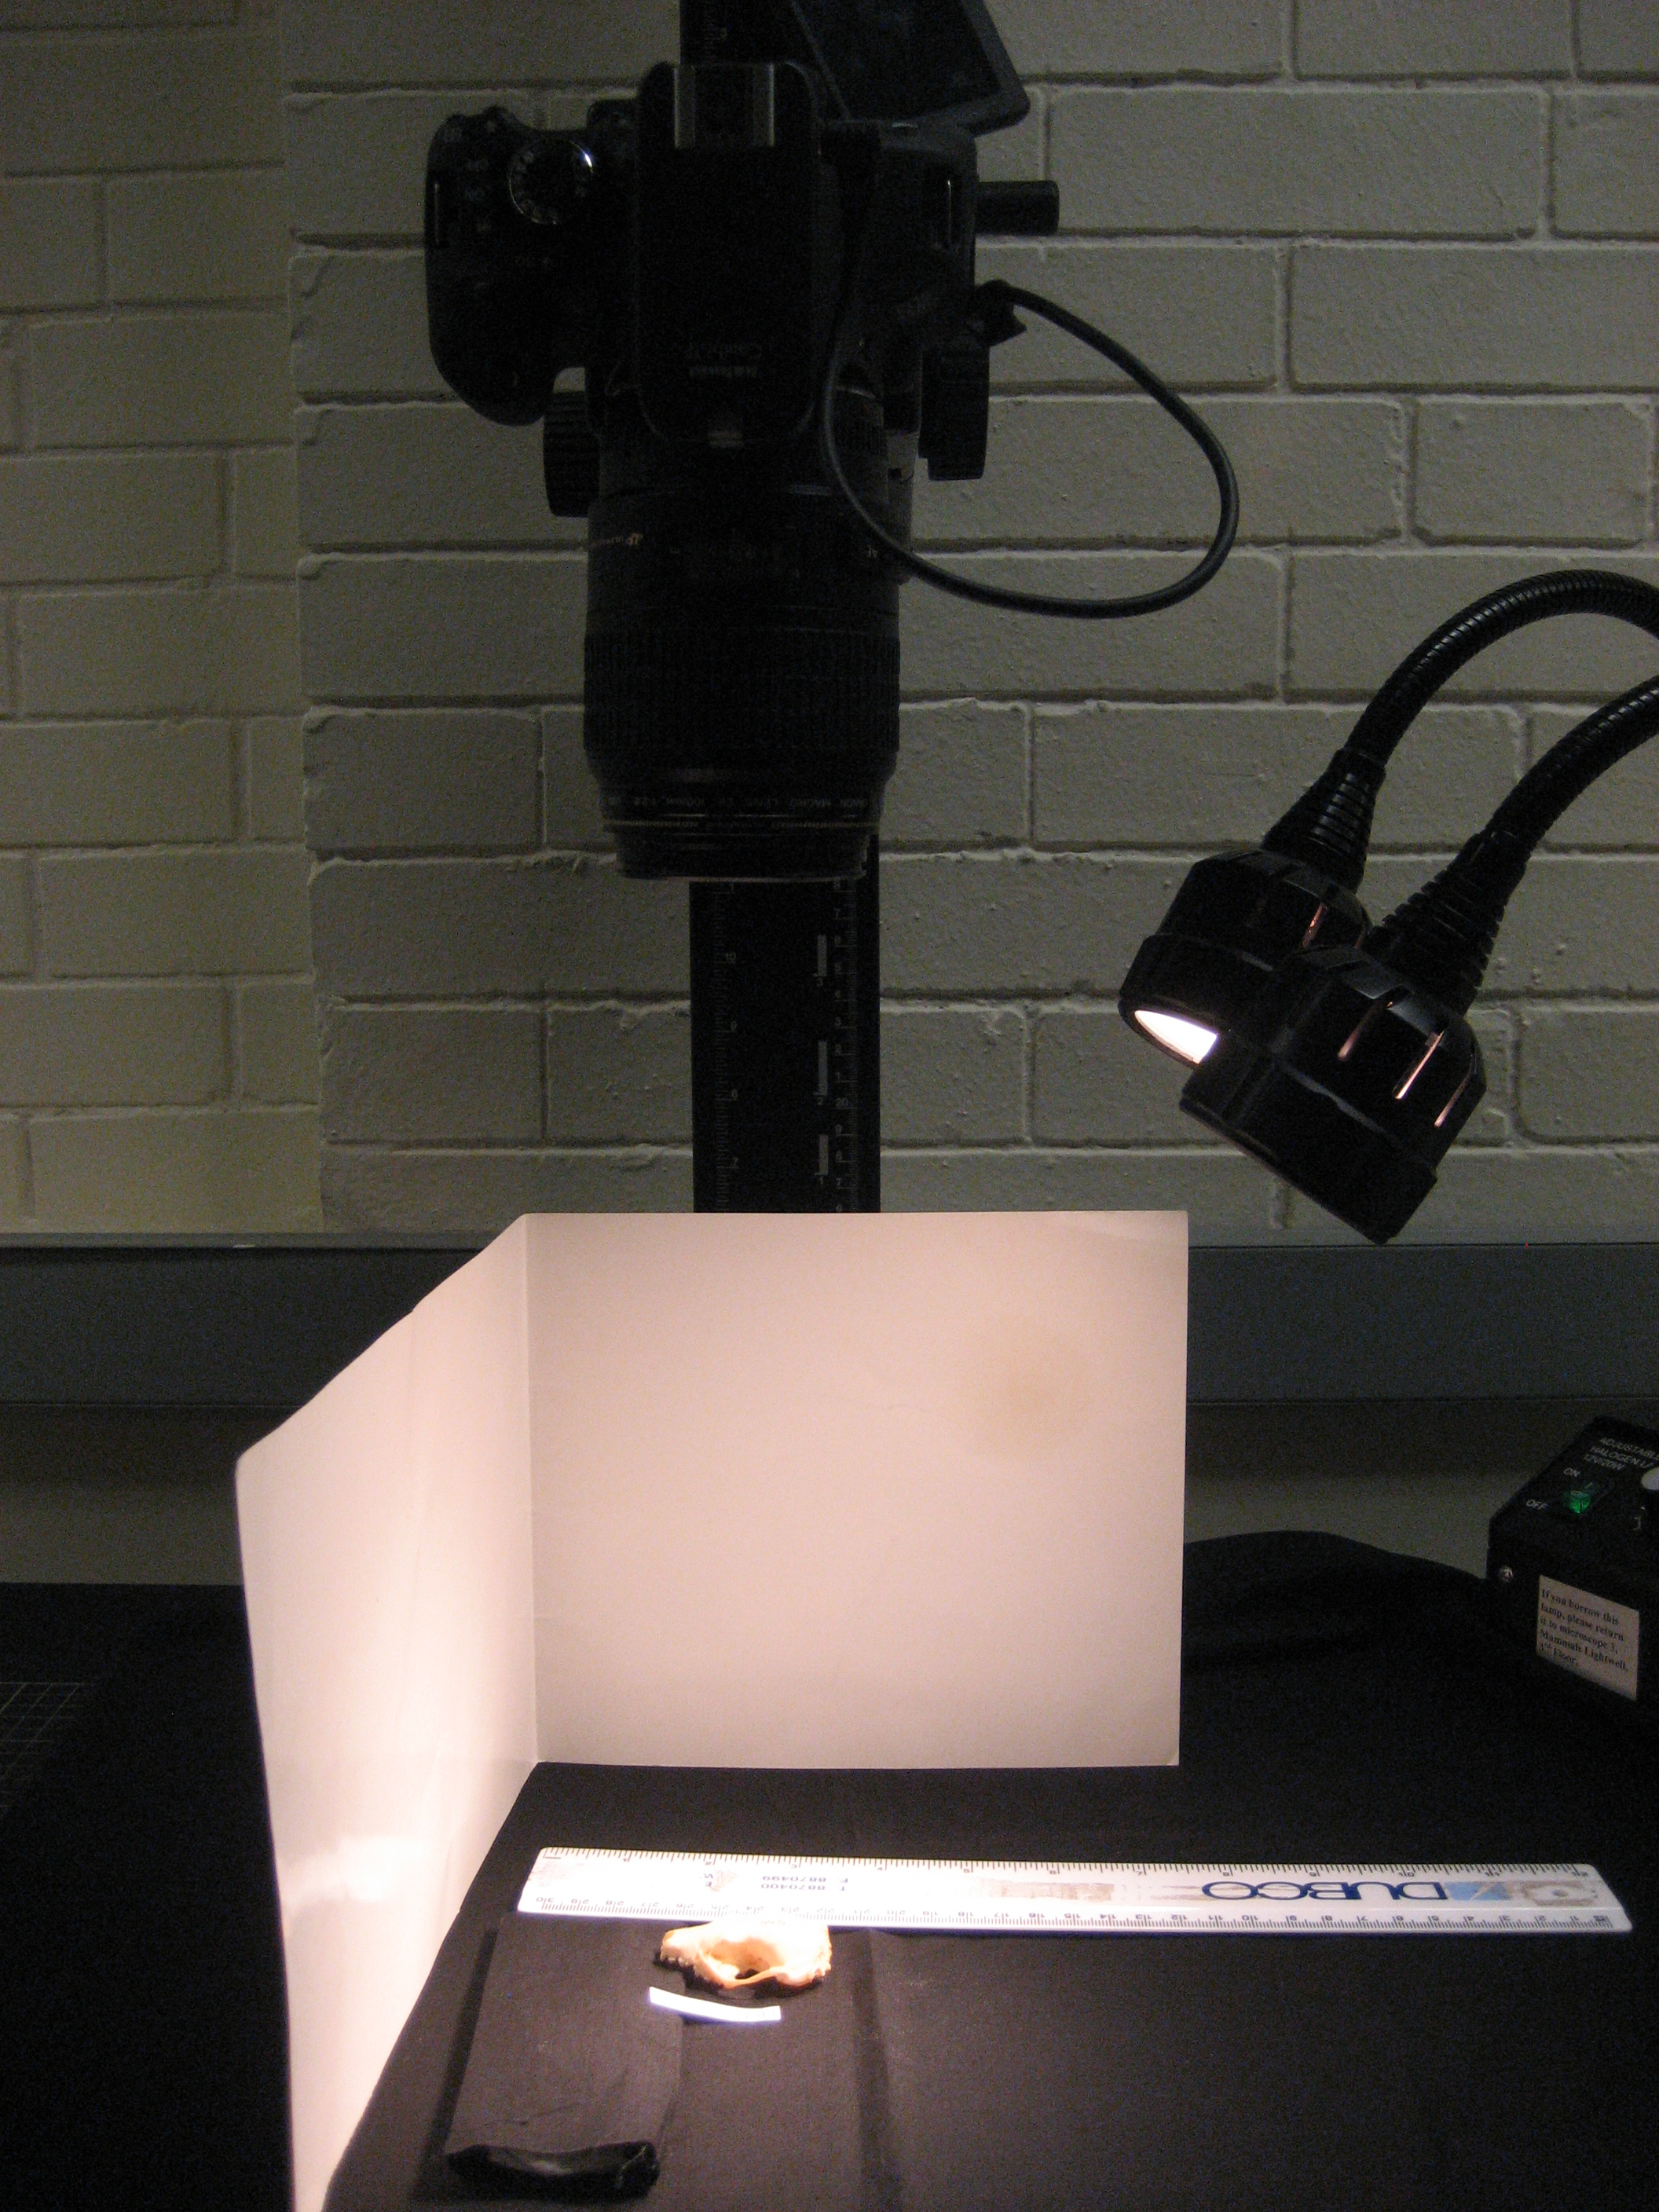
\includegraphics[width=12cm, height=12cm, keepaspectratio=true]{figures/camera.jpg}
    \caption[Photographic set up]%this is what appears in table of contents
    {Photographic set up for taking pictures of skulls. The camera (above centre) is fitted to a copy stand, the light source is directed from the top-left corner of the image and the white card reflects the light back onto the skull. }%this is under the figure
  	\label{fig:camera}
  	\end{figure}

Photographs were captured and saved in a raw file format. Before using the pictures for morphometric analyses, we converted the raw files to binary (grey scale) images and re-saved them as TIFF files. The black and white pictures were more useful for later analyses since we were not interested in including any colour comparisons and it is easier to see some biological features in binary images. TIFF files were the most appropriate to use for my morphometric analyses as they are uncompressed (in comparison to JPEG) images and therefore there is less chance of any picture distortions which may affect later analyses \citep{HERC2013}.
%----------------------------------------------
%Resampling for minimum number of points
%-----------------------------------------
\section{Determining the number of semilandmarks to use for curves}
	When combining landmark and semi-landmark approaches, there is a potential problem of over-sampling the curves \citep{Gunz2013}. To determine the number of semilandmark points required to adequately summarise the curves in our data sets,  we followed the method outlined by MacLeod \citeyearpar{MacLeod2012}. 
	For each data set we chose a random selection of pictures of specimens which represented the breadth of the morphological data (i.e. specimens from each sub-group of species).  We drew the appropriate curves on the each specimen and over-sampled the number of points on the curves (i.e. resampled the curves so that points were very close together). 
	We measured the length of the line and regarded that as the 100\%, true length of that outline. We then re-sampled the curves with decreasing numbers of points and measured the length of the outlines. We calculated the length of the curves resampled with fewere points as a percentage of the total length of the curve. We repeated these calculations for each specimen and then found the average percentage length for each resampled curve across all of the specimens in the test file. We continued this process until we found the minimum number of points that, on average, gave a curve length which was at least a 96\% accurate representatio of the true (over-sampled) curve length.  
	We repeated these curve-sampling tests for each analysis (skulls in dorsal/ventral/lateral views and mandibles in lateral view) to determine the minimum number of semilandmark points which would give accurate representations of morphological shape.

%---------------------------------------------------------
%Landmarks and results for ventral and lateral skull views
%---------------------------------------------------------
\section{Additional information for the morphometric analyses}

%--------------------------------------
\subsection{Landmark placement}

\subsubsection{Skulls: dorsal view}
	We placed ten landmarks and drew four semilandmark curves around the pictures of skulls in dorsal view (figure \ref{fig:skdors_landmarks} and table \ref{tab:skdors}). The curves summarise the shape of the braincase and palate.
	Given the absence of dental characteristics in this view, there were not many points which could be reliably identified across all of the species. Therefore we mainly relied on relative points (maximum width), the location of suture intersections and four semilandmark curves to summarise overall skull shape.  

%Skdors landmarks diagram
	\begin{figure}[!htb] 
 	\centering
  	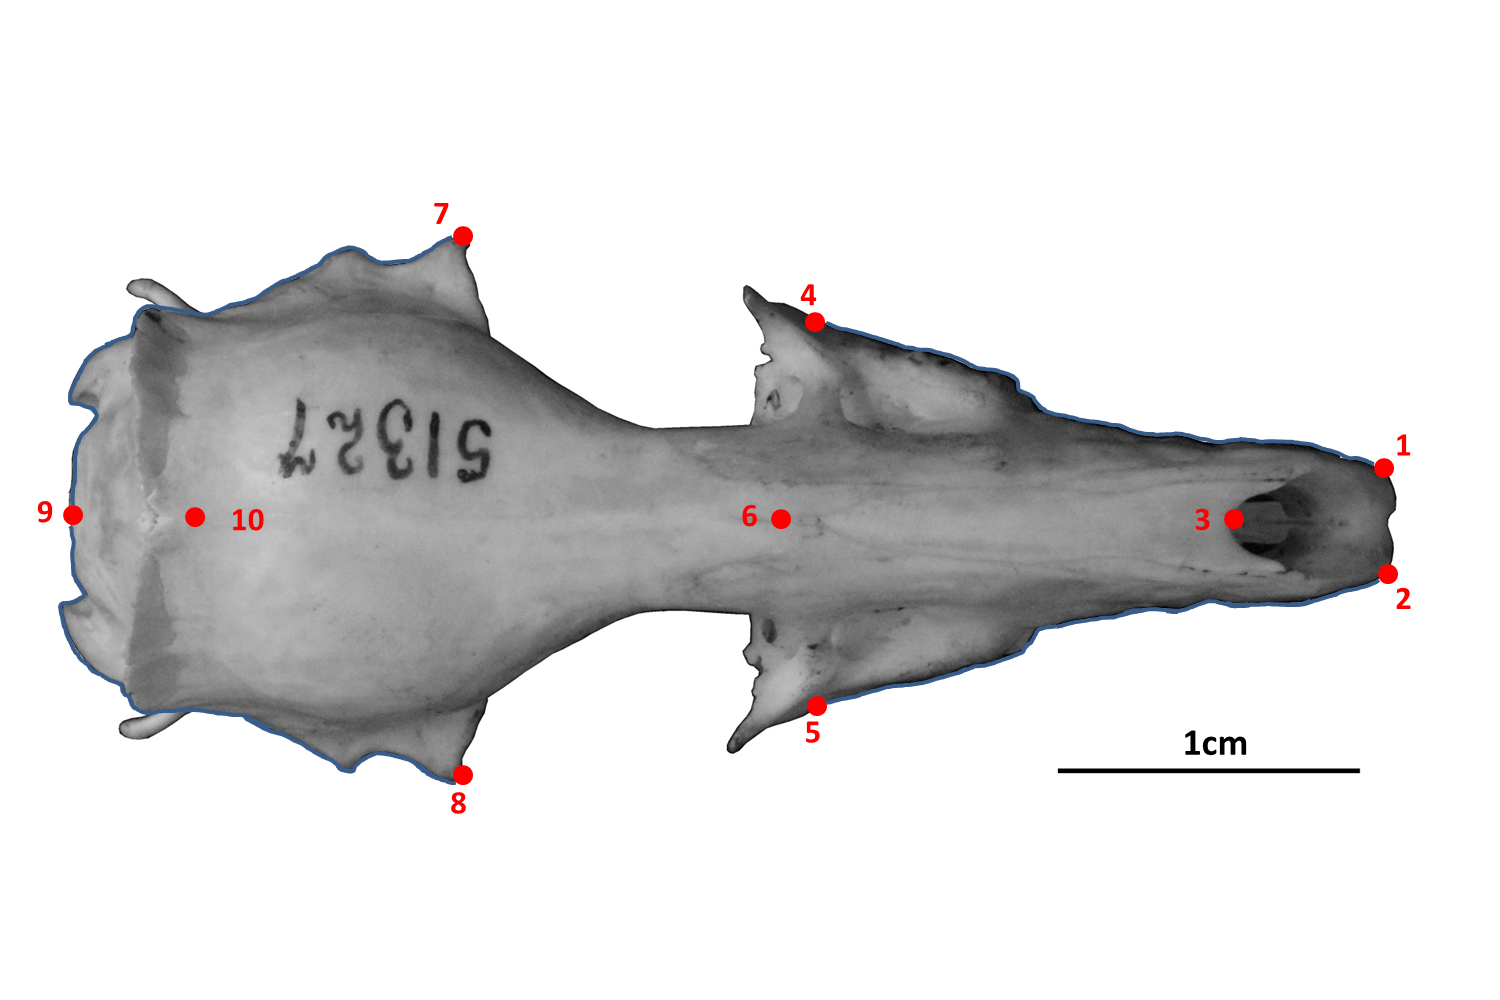
\includegraphics[width=12cm, height=12cm, keepaspectratio=true]
  	{figures/AMNH_51327_dorsallandmarksdiagram.png}    
    \caption {Landmarks (red) and curve (blue) for the dorsall skull pictures, further descriptions in table \ref{tab:skdors}. The specimen is a giant otter shrew tenrec, \textit{Potamogale velox}, AMNH 51327}
  	\label{fig:skdors_landmarks}
  	\end{figure}

%Table with skdors landmark descriptions
	\begin{table}[!htb]			
	\centering
	\caption{Descriptions of the landmarks (points) and curves (semilandmarks) for the skulls in dorsal view (see Figure \ref{fig:skdors_landmarks}).}
	%Skdors landmarks

\begin{tabular}[t]{l l}		
\hline
\textbf{Landmark} & \textbf{Description} \\
\hline
%------------------------------------------------------------
1 + 2 & Left (1) and right (2) anterior points of the premaxilla \\
%------------------------------------------------------------
3 & Anterior of the nasal bones in the midline \\
%------------------------------------------------------------
4 + 5 &	Maximum width of the palate (maxillary) on the left (4) and right (5)\\
%------------------------------------------------------------
6 & Midline intersection between nasal and frontal bones \\
%------------------------------------------------------------
7 + 8 & Widest point of the skull on the left (7) and right (8) \\
%------------------------------------------------------------
9 &	Posterior of the skull in the midline \\
	%Panchetti 2008 and Macholan2008 have different definitions for this one so I need to choose one
%------------------------------------------------------------
10 & Posterior intersection between saggital and parietal sutures \\
%--------------------------------------
\hline
\textbf{Curve A} & Outline of the braincase on the left side, between landmarks 9 and 7\\ 
(12 points) & (does not include visible features from the lower (ventral) side of the skull) \\

\textbf{Curve B} & Outline of the palate on the left side, between landamarks 4 and 1 \\
(10 points) & (outline of the rostrum only, not the shape of the teeth)\\

\textbf{Curve C} &	Outline of the braincase on the right side, between landmarks 9 and 8 \\
(12 points) & (does not include visible features from the lower (ventral) side of the skull) \\

\textbf{Curve D} & Outline of the palate on the right side, between landamarks 5 and 2 \\
(10 points) & (outline of the rostrum only, not the shape of the teeth)\\
%------------------------------------------------------------
\hline
\end{tabular} 
	\label{tab:skdors}  
	\end{table}

%--------------------------------------------------------------
\newpage
\subsubsection{Skulls: ventral view}
	Most of the landmarks in this view are concentrated around the dentition and palate of the animals. We placed 13 landmarks and drew one outline curve (resampled to 60 semilandmark points) around the back of the skulls between landmarks 12 and 13 (figure \ref{fig:skvent_landmarks}). The high variability of the species’ basi-cranial region and difficulties associated with identifying developmentally or functionally homologous points precluded designation of additional landmarks towards the back of the skulls. Table \ref{tab:skvent} outlines the descriptions of the landmarks we placed on the ventral pictures.


%Skvent diagram and landmarks description
	\begin{figure}[H] 
 	\centering
  	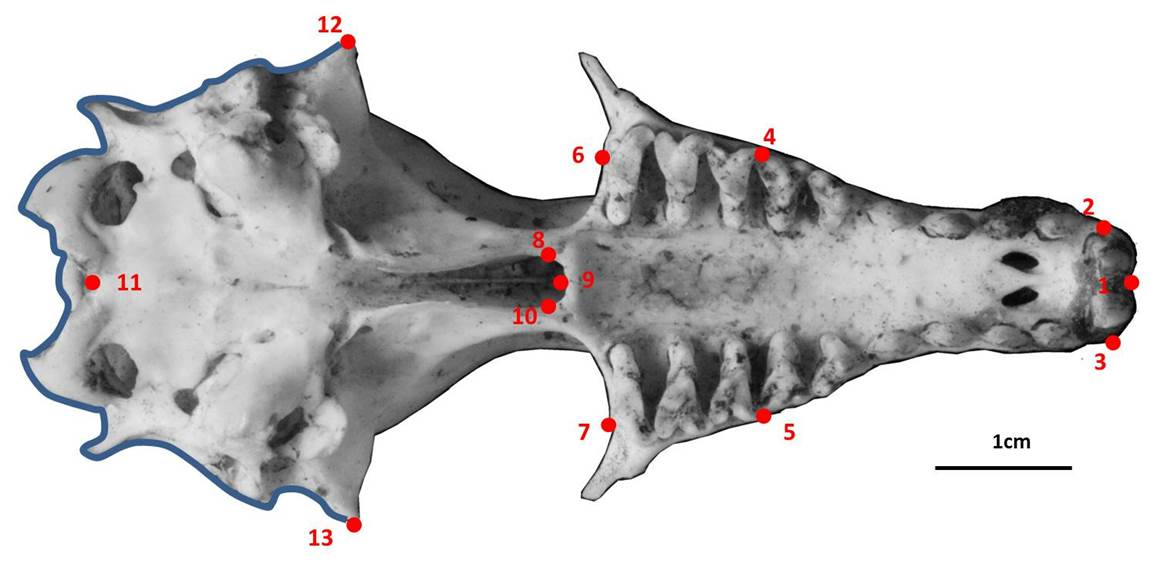
\includegraphics[width=12cm, height=12cm, keepaspectratio=true]
  	{figures/skvent_landmarks_pot_vel.jpg}
    \caption {Landmarks (red) and curve (blue) for the ventral skull pictures, further descriptions in table \ref{tab:skvent}. The specimen is a giant otter shrew tenrec, \textit{Potamogale velox}, NHML 1934.6.16.2}
  	\label{fig:skvent_landmarks}
  	\end{figure}


% Skulls ventral landmarks
	\begin{table}[h]
	\caption{Descriptions of the landmarks (points) and curves (semilandmarks) for the skulls in ventral view (see Figure \ref{fig:skvent_landmarks}.} 
	%SkVent landmarks
\begin{tabular}[t]{l l}		
\hline
\textbf{Landmark} & \textbf{Description} \\
\hline
%--------------------------------------
1 & Anterior point of the palate\\
%--------------------------------------
2 + 3 & Posterior, lateral extremity of the right (2) and left(3) incisor\\
%--------------------------------------
4 + 5 & Anterior, outer point of the first molar on the right (4) and left (5)\\
%--------------------------------------
6 + 7 & Posterior, outermost point of the molar surface on the right (6) and left (7) \\
%--------------------------------------
8 & Widest point of the curve of the palatine on the right side\\
%--------------------------------------
9 & Posterior point of the palatine in the midline\\
%--------------------------------------
10 & Widest point of the curve of the palatine on the left side\\
%--------------------------------------
11 & Anterior of the occipital foramen in the midline\\
%--------------------------------------
12 + 13 & Widest (extreme lateral) point of the braincase on the right (12) and left (13)\\
%--------------------------------------
Curve* & Outline of the back of the skull (between landmarks 12 and 13), 60 points \\
%------------------------------------------------------------
\hline
&*NB: This curve doesn't necessarily trace homologous features because of the \\ 
& variation in the position of the foramen magnum.
\end{tabular}
	\label{tab:skvent}
	\end{table}
	
%------------------------------------------------------
\subsubsection{Skulls: lateral view}
	We placed nine landmarks on the lateral pictures (see figure \ref{fig:sklat_landmarks}) and also drew two semilandmark curves between landmarks 7 and 8 to represent the shape of the back of the skull (resampled to 20 semilandmark points) and landmarks 8 and 1 (resampled to 15 semilandmark points) down the midline of the nose to represent the shape of the top of the skull. Table \ref{tab:sklat} describes the definitions for each of the landmark points. 
	For specimens that were damaged on their right side we reflected photographs of the left lateral side of the skull so that all pictures would be in the same orientation.

%Sklat diagram and landmarks description
	\begin{figure}[H] 
 	\centering
  	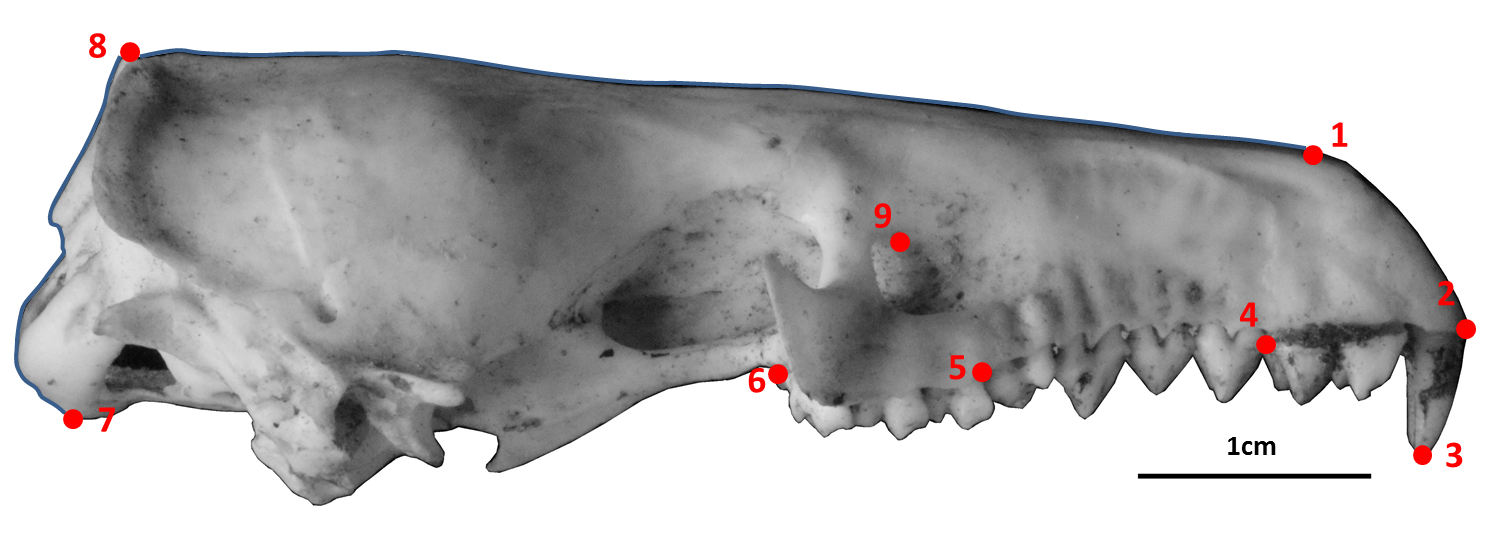
\includegraphics[width=12cm, height=12cm, keepaspectratio=true]
  	{figures/sklat_landmarks_pot_vel.png}
    \caption {Landmarks (red) and curve (blue) for the ventral skull pictures, further descriptions in table \ref{tab:skvent}. The specimen is a giant otter shrew tenrec, \textit{Potamogale velox}, NHML 1934.6.16.2}
  	\label{fig:sklat_landmarks}
  	\end{figure}


% Skulls lateral landmarks
	\begin{table}[h]
	\caption{Descriptions of the landmarks (points) and curves (semilandmarks) for the skulls in lateral view (see Figure \ref{fig:sklat_landmarks}.} 
	%Sklat landmarks
\begin{tabular}[t]{l l}		
\hline
\textbf{Landmark} & \textbf{Description} \\
\hline
%--------------------------------------
1 & Anterior, upper tip of the nasal bone\\
%--------------------------------------
2 & Anterior of the alveolus of the first incisor\\
%--------------------------------------
3 & Lowest point of the first incisor\\
%--------------------------------------
4& Posterior of the alveolus of the last incisor \\
%--------------------------------------
5 & Anterior tip of the alveolus of the first molar\\
%--------------------------------------
6 & Posterior tip of the alveolus of the last molar\\
%--------------------------------------
7 & Lowest point of the basi-occipital (base of the back of the skull)\\
%--------------------------------------
8 & Highest point of the braincase\\
%--------------------------------------
9 & Highest point of the infraorbital foramen\\
%--------------------------------------
\hline
\textbf{Curve A} & Between points 7 and 8  \\
(20 points)& Back of the skull from the lowest to highest points\\
%------------------------------------------------------------
\textbf{Curve B} & Between points 8 and 1  \\
(15 points)&From the highest point of the braincase to the front of the nasal \\
%------------------------------------------------------------
\hline
\end{tabular}
	\label{tab:sklat}
	\end{table}
%-------------------------------------------
\subsubsection{Mandibles}
	
	We placed seven landmarks and drew four outline curves around the mandible pictures (figure \ref{fig:mands_landmarks}, table \ref{tab:mands}). Curves A, B and C capture the shape of the condyloid, condylar and angular processes while curve D summarises the shape of the base of the jaw. For landmarks relying on identification of dental morphologies, we used a combination of published sources (REFS) to identify the dentitio of each species

%Mandibles landmark diagram
	\begin{figure}[H] 
 	\centering
  	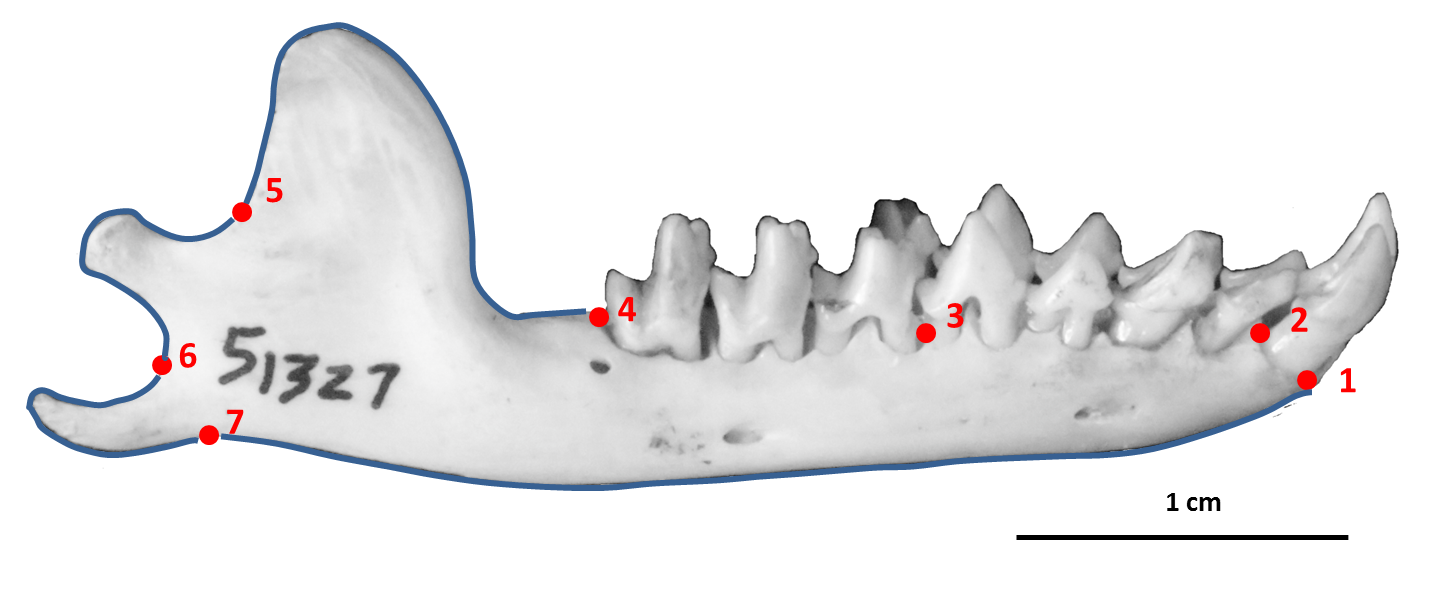
\includegraphics[width=12cm, height=12cm, keepaspectratio=true]
  	{figures/AMNH_51327_landmarksdiagram.png}
    \caption {Landmarks (red) and curve (blue) for the mandible pictures, further descriptions in table \ref{tab:mands}. The specimen is a giant otter shrew tenrec, \textit{Potamogale velox}, AMNH 51327}
  	\label{fig:mands_landmarks}
  	\end{figure}

%Table for the mandibles' landmark descriptions
	\begin{table}[h]			
	\centering
	\caption{Descriptions of the landmarks (points) and curves (semilandmarks) for the mandibles in lateral (buccal) view (see figure \ref{fig:mands_landmarks})}
	%Mandibles landmarks


\begin{tabular}[t]{l l}		
\hline
\textbf{Landmark} & \textbf{Description} \\
\hline
1 & Anterior of the alveolus of the first incisor \\
2 & Posterior of the alveolus of the first incisor \\
3 &	Anterior of the alveolus of the first molar \\
4 & Posterior of the alveolus of the last molar \\
5 & Maximum curvature between the coronoid and condylar processes\\
6 & Maximum curvature between the condylar and angular processes  \\
7 &	Maximum curvature between the angular process and the horizontal ramus \\
%---------------------------------------------------
\hline
Curve A & Condyloid process (between landmarks 4 and 5, 15 points)\\
Curve B & Condylar process (between landmarks 5 and 6, 15 points) \\
Curve C & Angular process (between landmarks 6 and 7, 15 points)  \\
Curve D & Base of the jaw (between landmarks 7 and 1, 12 points)  \\
%---------------------------------------------------
\hline
\end{tabular}


	\label{tab:mands} 
	\end{table}
%----------------------------------------------------------
\section{Additional mandible analyses}

	In our main analysis we found that golden moles had higher disparity in the shape of their mandibles compared to tenrecs. Our landmarks and curves for the mandibles emphasise shape variation in the ascending ramus of the mandible (figure \ref{fig:mands_landmarks}). We repeated our analyses with a reduced data set (deleted curves A, B and C table \ref{tab:mands}) to test whether higher variability in these posterior structures contributed to the apparently greater morphological variety within golden moles compared to tenrecs. Figure \ref{fig:mands_onecurvePCA} depicts the morphospace plot for this reduced-data analysis. Golden moles did not have higher disparity than tenrecs in this reduced-data analysis (table \ref{tab:mands_onecurve}). 

%Table for the results of the additional mandibles analysis
	\begin{table}[h]			
	\centering
	\caption{Results of our disparity comparisons for the reduced data set of mandibles (deleted curves A,B,C table \ref{tab:mands}). Permutation tests revealed no significant differences in disparity between the two families for any of the metrics (sum of variance, product of variance, sum of ranges, product of ranges, sum of squared distances between species and the overall mean shape). }
	%Disparity family comparison results summary
%Reduced mandibles data set: removed three of the four curves

\begin{tabular}[t]{l l l l }		
\hline
\textbf{Disparity metric} & \textbf{Tenrec} & \textbf{Golden mole} & \textbf{p value} \\ 
\hline
%-----------------------------------
SumVar & 0.0032 & 0.0063 & 0.29 \\
%-----------------------------------
ProdVar & 0.00053 & 0.00066 & 0.321 \\
%-----------------------------------
SumRange & 0.57 & 0.49 & 0.311 \\
%-----------------------------------
ProdRange & 0.11 & 0.08 & 0.384 \\
%-----------------------------------
SSqDist & 0.005 & 0.02 & 0 \\
\hline
\end{tabular}
	\label{tab:mands_onecurve} 
	\end{table}

%PCA plot for the reduced mandibles analyses	
	\begin{figure}[H] 
 	\centering
  	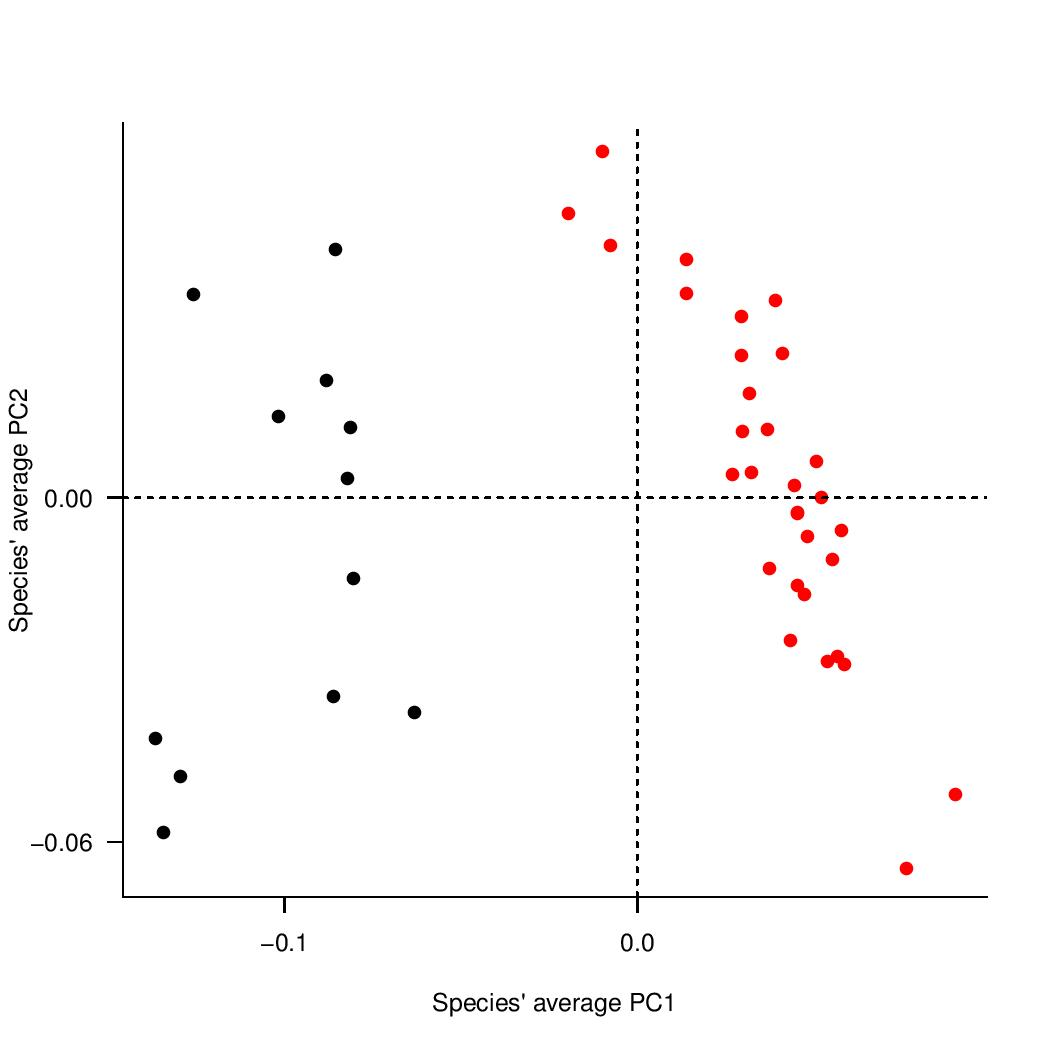
\includegraphics[width=12cm, height=12cm, keepaspectratio=true]
  	{figures/Mandibles_trc+gmole_onecurve_PCA.jpg}
    \caption {Principal components plot of the reduced data-set mandibles analysis (three of the curves removed). Each point represents the average mandible shape of an individual species of tenrec (red) and golden mole (black).}
  	\label{fig:mands_onecurvePCA}
  	\end{figure}

%---------------------------------------------------------
%Table of museum accession numbers
%---------------------------------------------------------
\section{Museum specimens}
	%I need to fix the position of the caption
	% Table generated by Excel2LaTeX from sheet 'Tenrec_Gmole_skulls_taxonomy'

%\documentclass[12pt]{article}
%\usepackage{longtable}
%\usepackage[margin ={1cm, 1cm, 1cm, 1cm, 1cm}]{geometry}
%\pagenumbering{}
%\begin{document}

%\begin{centre}
\begin{longtable}{|l|l|l|l|l|}

  \caption{Museum accession numbers and taxonomic identification for all skull specimens. AMNH (American Museum of Natural History), FMNH (Field Museum of Natural History), MCZ (Museum of Comparative Zoology, Harvard), NHML (Natural History Museum London), SI (Smithsonian Institute)}{l}\\
  \hline 

\textbf{Specimen ID} & \textbf{Order} & \textbf{Family} & \textbf{Genus} & \textbf{Species} \\
\hline
\endfirsthead

\multicolumn {5} {l}
{{\bfseries \tablename\ \thetable\ --\textit{Continues from previous page}}}\\
  \hline
  \textbf{SpecID} & \textbf{Order} & \textbf{Family} & \textbf{Genus} & \textbf{Species} \\
  \hline
\endhead

\hline \multicolumn{5}{|r|}{\textit{Continued on next page}} \\ 
\hline
\endfoot


\hline 
\endlastfoot

    AMNH\_161526 & Afrosoricida & Chrysochloridae & Chlorotalpa & duthieae \\
    AMNH\_161527 & Afrosoricida & Chrysochloridae & Chlorotalpa & duthieae \\
    AMNH\_161559 & Afrosoricida & Chrysochloridae & Eremitalpa & granti \\
    AMNH\_161571 & Afrosoricida & Chrysochloridae & Eremitalpa & granti \\
    AMNH\_167961 & Afrosoricida & Chrysochloridae & Chrysochloris & asiatica \\
    AMNH\_180911 & Afrosoricida & Chrysochloridae & Chrysochloris & stuhlmanni \\
    AMNH\_180912 & Afrosoricida & Chrysochloridae & Chrysochloris & stuhlmanni \\
    AMNH\_212938 & Afrosoricida & Tenrecidae & Hemicentetes & semispinosus \\
    AMNH\_274982 & Afrosoricida & Tenrecidae & Microgale & jobihely \\
    AMNH\_274986 & Afrosoricida & Tenrecidae & Microgale & jobihely \\
    AMNH\_274987 & Afrosoricida & Tenrecidae & Microgale & jobihely \\
    AMNH\_274988 & Afrosoricida & Tenrecidae & Microgale & jobihely \\
    AMNH\_274989 & Afrosoricida & Tenrecidae & Microgale & jobihely \\
    AMNH\_275041 & Afrosoricida & Tenrecidae & Microgale & soricoides \\
    AMNH\_275088 & Afrosoricida & Tenrecidae & Microgale & drouhardi \\
    AMNH\_275089 & Afrosoricida & Tenrecidae & Microgale & drouhardi \\
    AMNH\_275090 & Afrosoricida & Tenrecidae & Microgale & drouhardi \\
    AMNH\_275092 & Afrosoricida & Tenrecidae & Microgale & drouhardi \\
    AMNH\_275095 & Afrosoricida & Tenrecidae & Microgale & drouhardi \\
    AMNH\_275133 & Afrosoricida & Tenrecidae & Microgale & fotsifotsy \\
    AMNH\_275134 & Afrosoricida & Tenrecidae & Microgale & gymnorhyncha \\
    AMNH\_275135 & Afrosoricida & Tenrecidae & Microgale & gymnorhyncha \\
    AMNH\_275136 & Afrosoricida & Tenrecidae & Microgale & gymnorhyncha \\
    AMNH\_275137 & Afrosoricida & Tenrecidae & Microgale & gymnorhyncha \\
    AMNH\_275138 & Afrosoricida & Tenrecidae & Microgale & gymnorhyncha \\
    AMNH\_275141 & Afrosoricida & Tenrecidae & Microgale & longicaudata \\
    AMNH\_275142 & Afrosoricida & Tenrecidae & Microgale & longicaudata \\
    AMNH\_275143 & Afrosoricida & Tenrecidae & Microgale & longicaudata \\
    AMNH\_275148 & Afrosoricida & Tenrecidae & Microgale & longicaudata \\
    AMNH\_275149 & Afrosoricida & Tenrecidae & Microgale & longicaudata \\
    AMNH\_275157 & Afrosoricida & Tenrecidae & Microgale & parvula \\
    AMNH\_275158 & Afrosoricida & Tenrecidae & Microgale & soricoides \\
    AMNH\_275160 & Afrosoricida & Tenrecidae & Microgale & soricoides \\
    AMNH\_275162 & Afrosoricida & Tenrecidae & Microgale & soricoides \\
    AMNH\_275163 & Afrosoricida & Tenrecidae & Microgale & soricoides \\
    AMNH\_275189 & Afrosoricida & Tenrecidae & Oryzorictes & hova \\
    AMNH\_275190 & Afrosoricida & Tenrecidae & Oryzorictes & hova \\
    AMNH\_275191 & Afrosoricida & Tenrecidae & Oryzorictes & hova \\
    AMNH\_275250 & Afrosoricida & Tenrecidae & Microgale & brevicaudata \\
    AMNH\_275251 & Afrosoricida & Tenrecidae & Microgale & brevicaudata \\
    AMNH\_275253 & Afrosoricida & Tenrecidae & Microgale & brevicaudata \\
    AMNH\_275254 & Afrosoricida & Tenrecidae & Microgale & brevicaudata \\
    AMNH\_275255 & Afrosoricida & Tenrecidae & Microgale & brevicaudata \\
    AMNH\_275281 & Afrosoricida & Tenrecidae & Microgale & fotsifotsy \\
    AMNH\_275282 & Afrosoricida & Tenrecidae & Microgale & fotsifotsy \\
    AMNH\_275283 & Afrosoricida & Tenrecidae & Microgale & fotsifotsy \\
    AMNH\_275298 & Afrosoricida & Tenrecidae & Microgale & taiva \\
    AMNH\_275299 & Afrosoricida & Tenrecidae & Microgale & taiva \\
    AMNH\_275300 & Afrosoricida & Tenrecidae & Microgale & taiva \\
    AMNH\_275301 & Afrosoricida & Tenrecidae & Microgale & taiva \\
    AMNH\_275360 & Afrosoricida & Tenrecidae & Oryzorictes & hova \\
    AMNH\_275364 & Afrosoricida & Tenrecidae & Microgale & parvula \\
    AMNH\_275365 & Afrosoricida & Tenrecidae & Microgale & parvula \\
    AMNH\_275368 & Afrosoricida & Tenrecidae & Microgale & parvula \\
    AMNH\_31243 & Afrosoricida & Tenrecidae & Oryzorictes & tetradactylus \\
    AMNH\_31257 & Afrosoricida & Tenrecidae & Oryzorictes & tetradactylus \\
    AMNH\_31270 & Afrosoricida & Tenrecidae & Echinops & telfairi \\
    AMNH\_34647 & Afrosoricida & Chrysochloridae & Chrysospalax & trevelyani \\
    AMNH\_51324 & Afrosoricida & Tenrecidae & Potamogale & velox \\
    AMNH\_51327 & Afrosoricida & Tenrecidae & Potamogale & velox \\
    AMNH\_54365 & Afrosoricida & Chrysochloridae & Chrysospalax & trevelyani \\
    AMNH\_82399 & Afrosoricida & Chrysochloridae & Chrysochloris & stuhlmanni \\
    AMNH\_89040 & Afrosoricida & Chrysochloridae & Chrysospalax & trevelyani \\
    AMNH\_89046 & Afrosoricida & Chrysochloridae & Cryptochloris & wintoni \\
    FMNH\_156226 & Afrosoricida & Tenrecidae & Oryzorictes & tetradactylus \\
    FMNH\_159672 & Afrosoricida & Tenrecidae & Microgale & monticola \\
    FMNH\_159673 & Afrosoricida & Tenrecidae & Microgale & monticola \\
    FMNH\_159674 & Afrosoricida & Tenrecidae & Microgale & monticola \\
    FMNH\_159675 & Afrosoricida & Tenrecidae & Microgale & monticola \\
    FMNH\_159676 & Afrosoricida & Tenrecidae & Microgale & monticola \\
    FMNH\_162893 & Afrosoricida & Tenrecidae & Micropotamogale & lamottei \\
    FMNH\_166040 & Afrosoricida & Tenrecidae & Microgale & pusilla \\
    FMNH\_166111 & Afrosoricida & Tenrecidae & Microgale & gracilis \\
    FMNH\_166112 & Afrosoricida & Tenrecidae & Microgale & gracilis \\
    FMNH\_166113 & Afrosoricida & Tenrecidae & Microgale & gracilis \\
    FMNH\_166145 & Afrosoricida & Tenrecidae & Microgale & gracilis \\
    FMNH\_167427 & Afrosoricida & Tenrecidae & Microgale & dryas \\
    FMNH\_167621 & Afrosoricida & Tenrecidae & Microgale & pusilla \\
    FMNH\_176203 & Afrosoricida & Tenrecidae & Geogale & aurita \\
    FMNH\_176204 & Afrosoricida & Tenrecidae & Geogale & aurita \\
    FMNH\_176211 & Afrosoricida & Tenrecidae & Geogale & aurita \\
    FMNH\_176385 & Afrosoricida & Tenrecidae & Microgale & dryas \\
    FMNH\_176387 & Afrosoricida & Tenrecidae & Microgale & dryas \\
    FMNH\_176389 & Afrosoricida & Tenrecidae & Microgale & dryas \\
    FMNH\_176395 & Afrosoricida & Tenrecidae & Microgale & dryas \\
    FMNH\_209199 & Afrosoricida & Tenrecidae & Microgale & grandidieri \\
    FMNH\_209200 & Afrosoricida & Tenrecidae & Microgale & grandidieri \\
    FMNH\_209201 & Afrosoricida & Tenrecidae & Microgale & grandidieri \\
    FMNH\_209202 & Afrosoricida & Tenrecidae & Microgale & grandidieri \\
    FMNH\_209203 & Afrosoricida & Tenrecidae & Microgale & grandidieri \\
    FMNH\_53073 & Afrosoricida & Chrysochloridae & Amblysomus & corriae \\
    FMNH\_72831 & Afrosoricida & Tenrecidae & Potamogale & velox \\
    FMNH\_81731 & Afrosoricida & Chrysochloridae & Calcochloris & leucorhinus \\
    FMNH\_83540 & Afrosoricida & Chrysochloridae & Calcochloris & leucorhinus \\
    MCZ\_23373 & Afrosoricida & Chrysochloridae & Chrysochloris & stuhlmanni \\
    MCZ\_45021 & Afrosoricida & Tenrecidae & Oryzorictes & tetradactylus \\
    MCZ\_45022 & Afrosoricida & Tenrecidae & Oryzorictes & tetradactylus \\
    MCZ\_45033 & Afrosoricida & Tenrecidae & Microgale & pusilla \\
    MCZ\_45050 & Afrosoricida & Tenrecidae & Limnogale & mergulus \\
    MCZ\_45450 & Afrosoricida & Tenrecidae & Geogale & aurita \\
    MCZ\_46274 & Afrosoricida & Tenrecidae & Geogale & aurita \\
    NHML\_1870.3.10.15\_1527.a & Afrosoricida & Tenrecidae & Setifer & setosus \\
    NHML\_1934.6.16.2 & Afrosoricida & Tenrecidae & Potamogale & velox \\
    NHML\_1961.6.2.3 & Afrosoricida & Chrysochloridae & Chrysospalax & trevelyani \\
    NHML\_3.1.1.1 & Afrosoricida & Tenrecidae & Geogale & aurita \\
    NHML\_3.6.2.10 & Afrosoricida & Chrysochloridae & Amblysomus & hottentotus \\
    NHML\_3509 & Afrosoricida & Tenrecidae & Tenrec & ecaudatus \\
    NHML\_67.213 & Afrosoricida & Tenrecidae & Micropotamogale & ruwenzorii \\
    NHML\_73.170 & Afrosoricida & Tenrecidae & Micropotamogale & lamottei \\
    NHML\_74.668 & Afrosoricida & Chrysochloridae & Chrysochloris & sp. \\
    NHML\_75.2223 & Afrosoricida & Tenrecidae & Microgale & cowani \\
    NHML\_82.3.1.11 & Afrosoricida & Tenrecidae & Hemicentetes & nigriceps \\
    SI\_083658 & Afrosoricida & Tenrecidae & Hemicentetes & semispinosus \\
    SI\_154988 & Afrosoricida & Tenrecidae & Microgale & dobsoni \\
    SI\_154989 & Afrosoricida & Tenrecidae & Oryzorictes & tetradactylus \\
    SI\_221420 & Afrosoricida & Chrysochloridae & Chlorotalpa & duthieae \\
    SI\_266897 & Afrosoricida & Tenrecidae & Potamogale & velox \\
    SI\_294497 & Afrosoricida & Tenrecidae & Setifer & setosus \\
    SI\_294504 & Afrosoricida & Tenrecidae & Hemicentetes & semispinosus \\
    SI\_294507 & Afrosoricida & Tenrecidae & Hemicentetes & nigriceps \\
    SI\_294508 & Afrosoricida & Tenrecidae & Hemicentetes & nigriceps \\
    SI\_294510 & Afrosoricida & Tenrecidae & Hemicentetes & nigriceps \\
    SI\_294511 & Afrosoricida & Tenrecidae & Hemicentetes & nigriceps \\
    SI\_294520 & Afrosoricida & Tenrecidae & Microgale & dobsoni \\
    SI\_328604 & Afrosoricida & Tenrecidae & Setifer & setosus \\
    SI\_328605 & Afrosoricida & Tenrecidae & Setifer & setosus \\
    SI\_328614 & Afrosoricida & Tenrecidae & Setifer & setosus \\
    SI\_328616 & Afrosoricida & Tenrecidae & Echinops & telfairi \\
    SI\_328619 & Afrosoricida & Tenrecidae & Echinops & telfairi \\
    SI\_328622 & Afrosoricida & Tenrecidae & Echinops & telfairi \\
    SI\_328624 & Afrosoricida & Tenrecidae & Echinops & telfairi \\
    SI\_328653 & Afrosoricida & Tenrecidae & Microgale & cowani \\
    SI\_328662 & Afrosoricida & Tenrecidae & Microgale & cowani \\
    SI\_328667 & Afrosoricida & Tenrecidae & Microgale & cowani \\
    SI\_328669 & Afrosoricida & Tenrecidae & Microgale & cowani \\
    SI\_328670 & Afrosoricida & Tenrecidae & Microgale & cowani \\
    SI\_328688 & Afrosoricida & Tenrecidae & Microgale & pusilla \\
    SI\_328689 & Afrosoricida & Tenrecidae & Microgale & pusilla \\
    SI\_328690 & Afrosoricida & Tenrecidae & Microgale & pusilla \\
    SI\_328695 & Afrosoricida & Tenrecidae & Microgale & dobsoni \\
    SI\_341621 & Afrosoricida & Tenrecidae & Tenrec & ecaudatus \\
    SI\_341624 & Afrosoricida & Tenrecidae & Tenrec & ecaudatus \\
    SI\_341661 & Afrosoricida & Tenrecidae & Hemicentetes & semispinosus \\
    SI\_341688 & Afrosoricida & Tenrecidae & Hemicentetes & semispinosus \\
    SI\_341689 & Afrosoricida & Tenrecidae & Hemicentetes & semispinosus \\
    SI\_351334 & Afrosoricida & Chrysochloridae & Calcochloris & obtusirostris \\
    SI\_351335 & Afrosoricida & Chrysochloridae & Calcochloris & obtusirostris \\
    SI\_351336 & Afrosoricida & Chrysochloridae & Chrysospalax & villosus \\
    SI\_351955 & Afrosoricida & Chrysochloridae & Calcochloris & obtusirostris \\
    SI\_361482 & Afrosoricida & Tenrecidae & Tenrec & ecaudatus \\
    SI\_365001 & Afrosoricida & Chrysochloridae & Carpitalpa & arendsi \\
    SI\_380484 & Afrosoricida & Chrysochloridae & Amblysomus & hottentotus \\
    SI\_380485 & Afrosoricida & Chrysochloridae & Amblysomus & hottentotus \\
    SI\_381488 & Afrosoricida & Chrysochloridae & Amblysomus & hottentotus \\
    SI\_395676 & Afrosoricida & Tenrecidae & Geogale & aurita \\
    SI\_449177 & Afrosoricida & Tenrecidae & Microgale & taiva \\
    SI\_449179 & Afrosoricida & Tenrecidae & Microgale & gracilis \\
    SI\_449192 & Afrosoricida & Tenrecidae & Microgale & dobsoni \\
    SI\_468315 & Afrosoricida & Chrysochloridae & Chrysochloris & asiatica \\
    SI\_468316 & Afrosoricida & Chrysochloridae & Chrysochloris & asiatica \\
    SI\_468317 & Afrosoricida & Chrysochloridae & Chrysochloris & asiatica \\
    SI\_468318 & Afrosoricida & Chrysochloridae & Eremitalpa & granti \\
    SI\_468319 & Afrosoricida & Chrysochloridae & Cryptochloris & wintoni \\
    SI\_470211 & Afrosoricida & Chrysochloridae & Calcochloris & obtusirostris \\
    SI\_537651 & Afrosoricida & Tenrecidae & Potamogale & velox \\
    SI\_577052 & Afrosoricida & Tenrecidae & Oryzorictes & hova \\
    SI\_577055 & Afrosoricida & Tenrecidae & Microgale & talazaci \\
    SI\_578746 & Afrosoricida & Tenrecidae & Microgale & talazaci \\
    SI\_578747 & Afrosoricida & Tenrecidae & Microgale & talazaci \\
    SI\_578749 & Afrosoricida & Tenrecidae & Microgale & dobsoni \\
    SI\_578753 & Afrosoricida & Tenrecidae & Microgale & principula \\
    SI\_578756 & Afrosoricida & Tenrecidae & Microgale & principula \\
    SI\_578759 & Afrosoricida & Tenrecidae & Microgale & principula \\
    SI\_578760 & Afrosoricida & Tenrecidae & Microgale & principula \\
    SI\_578762 & Afrosoricida & Tenrecidae & Microgale & principula \\
    SI\_578768 & Afrosoricida & Tenrecidae & Microgale & talazaci \\
    SI\_578769 & Afrosoricida & Tenrecidae & Microgale & talazaci \\
    SI\_578772 & Afrosoricida & Tenrecidae & Microgale & thomasi \\
    SI\_578773 & Afrosoricida & Tenrecidae & Microgale & thomasi \\
    SI\_578774 & Afrosoricida & Tenrecidae & Microgale & thomasi \\
    SI\_578775 & Afrosoricida & Tenrecidae & Microgale & thomasi \\
    SI\_578776 & Afrosoricida & Tenrecidae & Microgale & thomasi \\
    SI\_578784 & Afrosoricida & Tenrecidae & Microgale & parvula \\
    SI\_578787 & Afrosoricida & Tenrecidae & Microgale & fotsifotsy \\
    SI\_578789 & Afrosoricida & Tenrecidae & Oryzorictes & sp. \\
    SI\_578791 & Afrosoricida & Tenrecidae & Tenrec & ecaudatus \\
    SI\_578792 & Afrosoricida & Tenrecidae & Tenrec & ecaudatus \\
    SI\_584649 & Afrosoricida & Chrysochloridae & Calcochloris & leucorhinus \\

\end{longtable}
%\end{centre}
%\end{document}

	%  \label{tab:sk.taxonomy}%
	%\end{table}%

\bibliographystyle{jeb}
\bibliography{refs_disparity}
\end{document}